\documentclass[11pt]{article}

\usepackage[a4paper,margin=1in]{geometry}
\usepackage{amsmath,amssymb,amsfonts}
\usepackage{booktabs}
\usepackage{longtable}
\usepackage{array}
\usepackage{graphicx}
\usepackage{xcolor}
\usepackage{hyperref}
\usepackage{enumitem}
\usepackage{caption}
\usepackage{float}
\usepackage{fontspec}
\usepackage{xeCJK}

\setmainfont{Helvetica Neue}
\setsansfont{Helvetica Neue}
\setmonofont{Menlo}
\setCJKmainfont{PingFang SC}
\setCJKsansfont{PingFang SC}
\setCJKmonofont{PingFang SC}

\graphicspath{{../figures/}}

\hypersetup{
  colorlinks=true,
  linkcolor=blue!50!black,
  citecolor=blue!50!black,
  urlcolor=blue!50!black
}

\newcommand{\R}{\mathbb{R}}
\newcommand{\V}{\mathcal{V}}
\newcommand{\E}{\mathcal{E}}
\newcommand{\WCA}{\mathrm{WCA}}
\newcommand{\diag}{\operatorname{diag}}
\newcommand{\MSE}{\operatorname{MSE}}
\renewcommand{\abstractname}{摘要}
\renewcommand{\contentsname}{目录}

\title{\textbf{World Cellular Automata}\\
\large 面向世界状态建模的递归局部世界架构\\
\normalsize 技术报告 v0.1}
\author{WCA Research Project}
\date{2026-07-01}

\begin{document}
\maketitle

\begin{abstract}
World Cellular Automata（WCA）是一种面向世界状态建模的递归架构。它不把当前观测直接映射为未来场，而是先把全局状态展开为一族以节点为中心的局部世界，在局部世界内部通过学习到的成对交互进行演化，再把演化后的中心重新组合为下一步全局状态。本文从有限集合语义和张量语义出发，给出 WCA 的架构动机、实验金字塔和当前证据。核心观点是：递归的局部世界综合可以作为一种可检验、可归因的世界状态预测计算基底。目前最强证据来自 PDEBench reaction-diffusion 的 token-level 实验；递归深度、可学习场接口、归因控制实验和 h8x2 rollout 共同表明，WCA core 在若干长程预测设置中能够贡献超过接口本身和无递归控制组的有效信号。本文同时记录失败模式和边界，包括 PatchMean 接口瓶颈、N=256 PatchMean 扩展失败、native/full-field 视觉细节不足以及 dense 实现的系统成本。这些不是结论的终点，而是下一阶段研究路线的起点。
\end{abstract}

\tableofcontents
\newpage

\section{范围与用途}

本文不是压缩投稿稿，而是一份公开研究记录。目标是完整呈现 WCA 的架构、实验、证据、失败模式和未来路线，便于发布到 GitHub、Hugging Face 和 Zenodo。它不追求短，而追求清楚、完整、可追溯。

本文不使用传统算法伪代码作为主要说明方式。WCA 的核心不是一个普通训练 loop，而是中间张量 $L$ 的语义：每个中心节点拥有一个局部世界，局部世界内部发生 receiver-sender pair evolution，最后只取演化后的中心重新组合成下一步世界状态。用普通伪代码很容易把 WCA 写得像 GNN 或普通 NCA，因此本文采用数学定义、shape contract、计算图和实验证据树来表达。

\section{为什么研究 WCA}

物理预测和具身预测任务同时需要局部交互和全局一致性。反应扩散、接触动力学、热扩散、路径规划和天气场都可以看成局部规则不断积累形成全局状态的过程。直接场预测模型可以很强，但它常常把状态演化机制藏在一个从输入到输出的黑盒映射里。传统细胞自动机有清晰的局部规则，但纯局部规则很难长期维持全局上下文。

WCA 尝试走中间路线。每个节点都构造一个以自己为中心的局部世界；局部世界内部通过成对关系演化；演化后的中心再回到共享世界状态。它的基本结构是：

\[
H_t \longrightarrow L_t \longrightarrow L'_t \longrightarrow H_{t+1}.
\]

这个设计背后的判断是：

\begin{quote}
如果模型能够反复把全局状态分化为局部世界，再把演化后的局部世界重新综合成全局状态，那么它可能学习到有用的世界状态动力学。
\end{quote}

这个判断是可以被证伪的。如果递归深度没有帮助、outer0 无递归控制组与完整 WCA 一样强、tokenizer-only 控制组解释了全部收益，或者长程 rollout 崩溃，那么 WCA 假设就会变弱。因此本文的实验不是简单追逐单一分数，而是围绕这些证伪条件建立证据树。

\section{数学定义}

\subsection{世界状态}

设世界由有限节点集表示：

\[
\V = \{1,2,\ldots,N\}.
\]

在时间 $t$，WCA 的世界状态可以写成函数：

\[
h_t:\V \rightarrow \R^D,
\]

对应批量张量：

\[
H_t \in \R^{B \times N \times D}.
\]

其中 $B$ 是 batch size，$N$ 是节点或场 token 数，$D$ 是隐藏维度。

\subsection{局部世界族}

WCA 的关键动作是把全局世界状态展开成一族局部世界：

\[
L_t = \Pi_\theta(H_t), \qquad
L_t \in \R^{B \times N_c \times N_v \times D}.
\]

在 protected dense baseline 中，$N_c=N_v=N$。第一个节点轴表示局部世界中心 $c$，第二个节点轴表示该中心局部世界中被表示的节点 $r$。函数形式为：

\[
\ell_{t,c}: \V \rightarrow \R^D,
\qquad
\{\ell_{t,c}\}_{c\in \V}.
\]

这正是 WCA 与普通 message passing 的区别。普通 GNN 主要更新节点 $i$；WCA 则让每个中心 $c$ 持有一个完整的局部世界解释，然后在这些局部世界内部进行演化。

\subsection{局部世界内部的成对演化}

在以 $c$ 为中心的局部世界中，receiver 节点 $r$ 从 sender 节点 $s$ 聚合成对交互：

\[
\ell^{k+1}_{t,c}(r)
=
\ell^{k}_{t,c}(r)
+
\sum_{s\in \V}
A_{rs}\,
\phi_\theta
\left(
\ell^{k}_{t,c}(r),
\ell^{k}_{t,c}(s),
e_{rs}
\right).
\]

其中 $A_{rs}$ 是邻接或支持权重，$e_{rs}$ 是可选边特征，$\phi_\theta$ 是学习到的 pair kernel，$k$ 是 inner pair-evolution step。完整 dense 语义等价于：

\[
[B,N,N,N,D],
\]

也就是 batch、center、receiver、sender 和 hidden channel 五个维度。实现可以 chunk 或重排计算，但不能在 baseline 中悄悄去掉 center 语义。

\subsection{中心重组}

经过 $K$ 次内部演化后，WCA 从演化后的中心对角线重组下一步世界状态：

\[
h_{t+1}(i)
=
\rho_\theta\left(\ell^{K}_{t,i}(i)\right),
\]

也可以写成：

\[
H_{t+1}
=
\rho_\theta\left(\diag L_t^K\right).
\]

所以 center index 不是实现细节，而是语义载体。以 $i$ 为中心的局部世界中，节点 $i$ 的演化表示被写回下一步全局状态。

\subsection{外层递归}

一次 WCA 更新可以继续递归展开：

\[
H_{t}^{(m+1)}
=
F_\theta\left(H_t^{(m)}, A, E\right),
\qquad
m=0,\ldots,M-1.
\]

实验中的 outer recursion depth 就是 $M$。V25 recursion ladder 正是在测试更深的递归是否改善长程预测。

\section{Shape Contract 与结构不变量}

\begin{longtable}{p{0.22\linewidth}p{0.28\linewidth}p{0.40\linewidth}}
\toprule
对象 & 形状 & 含义 \\
\midrule
$H_t$ & $[B,N,D]$ & 时间 $t$ 的全局世界状态。 \\
$L_t$ & $[B,N,N,D]$ & 以中心节点索引的局部世界族。 \\
Pair 语义 & $[B,N,N,N,D]$ & batch、center、receiver、sender、channel。 \\
$\diag L_t$ & $[B,N,D]$ & 用于重组的演化中心。 \\
$H_{t+1}$ & $[B,N,D]$ & 下一步全局世界状态。 \\
\bottomrule
\end{longtable}

WCA baseline 必须保持以下不变量：

\begin{enumerate}[leftmargin=2em]
  \item 维护世界状态 $H_t\in\R^{B\times N\times D}$。
  \item 构造局部世界 $L_t\in\R^{B\times N\times N\times D}$。
  \item pair evolution 在局部世界内部发生，并保留 center index。
  \item 重组时取演化后的中心生成 $H_{t+1}$。
  \item 内存优化必须保持 dense 语义；如果改变语义，必须作为显式变体或 ablation。
\end{enumerate}

\begin{figure}[H]
\centering
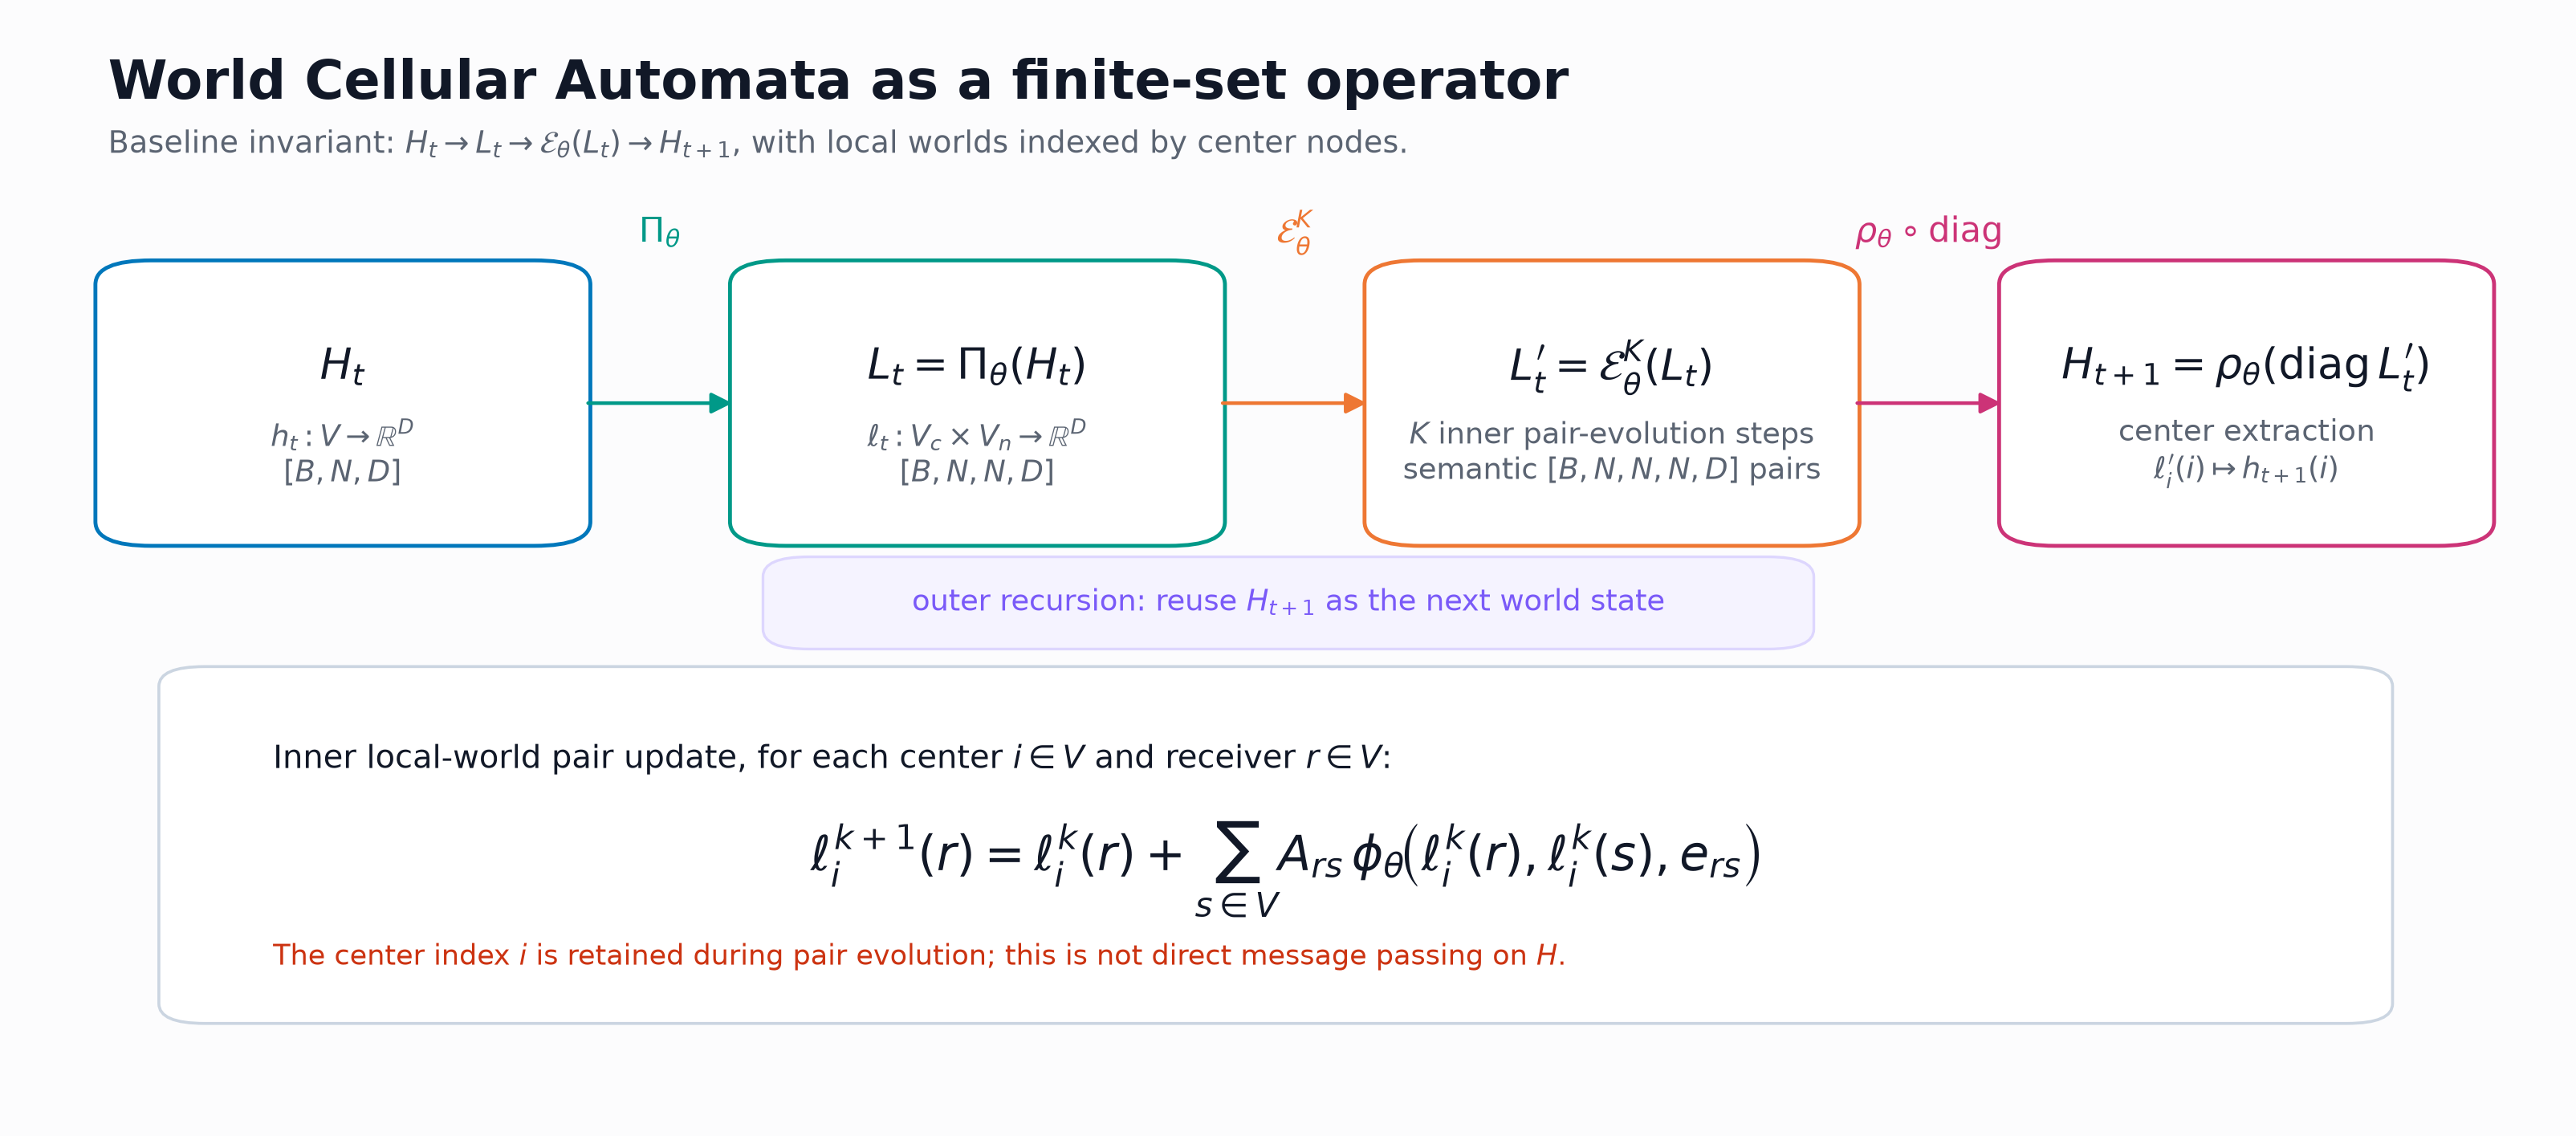
\includegraphics[width=0.95\linewidth]{wca_formal_operator_diagram.png}
\caption{WCA 的有限集合算子视角。核心不变量是 $H_t \rightarrow L_t \rightarrow \mathcal{E}_\theta(L_t) \rightarrow H_{t+1}$。}
\end{figure}

\begin{figure}[H]
\centering
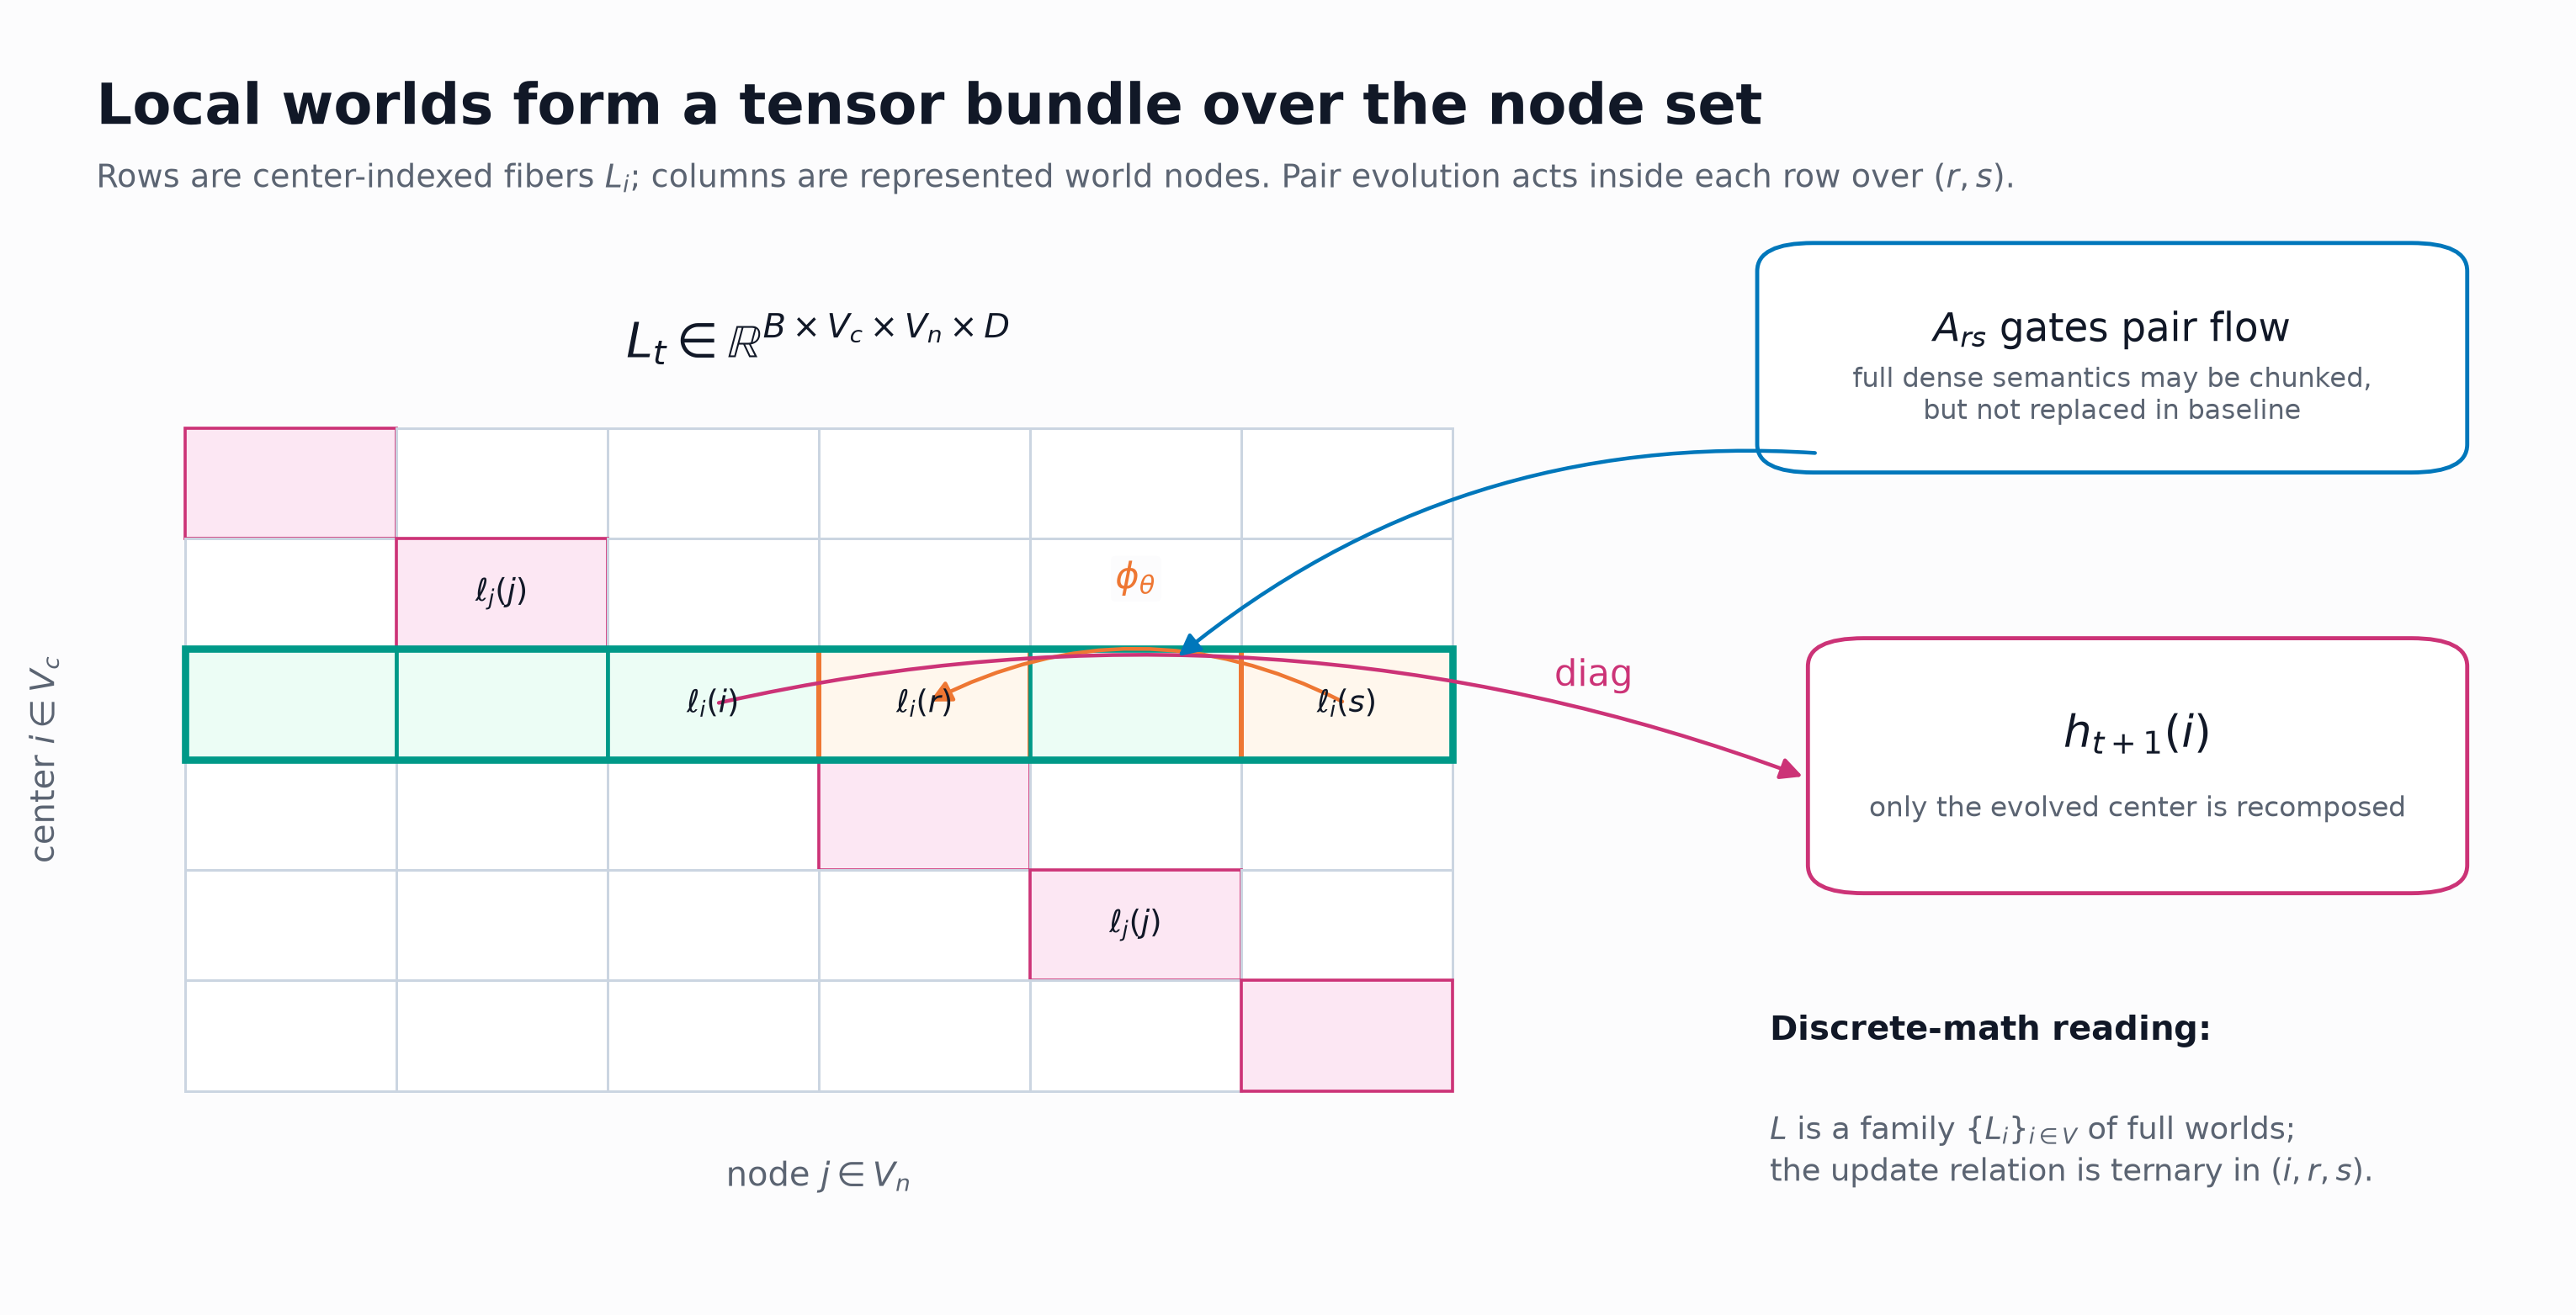
\includegraphics[width=0.95\linewidth]{wca_formal_tensor_fiber_diagram.png}
\caption{局部世界形成定义在节点集上的张量束。pair evolution 在 center-indexed row 内部作用于 $(r,s)$。}
\end{figure}

\section{与其他模型族的关系}

\subsection{与 Neural CA 的关系}

Neural CA 学习局部更新规则，说明重复局部变换可以生成全局结构。WCA 继承了这一思想，但它不是简单在网格邻域上更新单个 cell。每个中心 $c$ 都持有一个完整局部世界 $\ell_c$，pair evolution 在该局部世界内部发生，最后再取中心重组。

\subsection{与 GNN 的关系}

普通 GNN 可写作：

\[
h_i^{+}
=
\psi_\theta
\left(
h_i,
\sum_{j\in \mathcal{N}(i)}
\phi_\theta(h_i,h_j,e_{ij})
\right).
\]

WCA 则写作：

\[
\ell_c(r)^{+}
=
\ell_c(r)
+
\sum_s A_{rs}\phi_\theta(\ell_c(r),\ell_c(s),e_{rs}).
\]

多出来的 center index $c$ 是关键。去掉它，模型就会退化到普通 message passing。因此这种退化只能作为 ablation，不能当作等价实现。

\subsection{与 Transformer Attention 的关系}

Transformer attention 通过 query-key-value 计算 token 间的加权交互。WCA 也学习节点关系，但核心不是标准 attention block，而是局部世界构造、局部世界内部演化和中心重组。未来可以把 attention 风格组件作为 pair kernel 变体，但那不是当前 protected baseline。

\subsection{与 Neural Operator 的关系}

Neural operator 学习函数空间之间的映射，是 PDE surrogate modeling 的强基线。WCA 不是要取代 FNO，而是提出另一个问题：递归局部世界状态机是否能学到有用的世界动力学？因此本文的重点不是单纯比榜，而是验证 WCA core 是否在控制接口和无递归替代后仍有贡献。

\section{接口：从数据到世界 token}

WCA 当前吃的是向量化状态 token，不是 NLP 文本 token。场、迷宫或未来多模态状态都需要被编码成 $H_t$。

\subsection{Maze 接口}

迷宫中，节点对应网格 cell。输入包含墙、起点、终点、坐标和 open-cell 信息。输出是 potential field 或 distance-like field，用于 greedy path rollout。评价不能只看 MSE，而要看 path success、path optimal、loop rate、goal rank、local minima 等功能指标。

\subsection{PatchMean 场接口}

对于场：

\[
X_t \in \R^{C \times H \times W},
\]

PatchMean 将场切成 $N$ 个 patch，并对每个 patch 求均值：

\[
z_i
=
\frac{1}{|\Omega_i|}
\sum_{(u,v)\in \Omega_i}
X_t(:,u,v).
\]

这种接口简单可审计，但会丢掉 patch 内结构，尤其影响 h1/h2 这种短期预测。

\subsection{可学习 patch 接口}

可学习接口把均值替换为：

\[
z_i = g_\eta(X_t|_{\Omega_i}),
\]

其中 $g_\eta$ 可以是 MLP stem 或 Conv stem。它能保留更多局部结构，但也会带来归因问题：提升到底来自接口，还是来自 WCA core？因此需要 tokenizer-only、outer0、token MLP 和 token Conv 控制组。

\section{训练目标与指标}

监督场预测使用 MSE：

\[
\mathcal{L}_{\mathrm{MSE}}
=
\frac{1}{|\Omega|}
\sum_{q\in \Omega}
\left(
\hat{Y}_{t+h}(q)-Y_{t+h}(q)
\right)^2.
\]

Relative $L^2$ error 定义为：

\[
\mathrm{RelL2}
=
\frac{\|\hat{Y}_{t+h}-Y_{t+h}\|_2}
{\|Y_{t+h}\|_2+\epsilon}.
\]

对于 token-level WCA，formal metric 是 token-space MSE。patch-repeated 图像看起来会更块状，但这不等于 token-level metric 错；同时，full-field baseline 图像更细腻，也不自动说明它在 token contract 下更强。metric space 必须明确。

\section{证据树}

WCA 项目按照证据树推进，而不是按灵感随意跑实验。

\begin{longtable}{p{0.18\linewidth}p{0.34\linewidth}p{0.38\linewidth}}
\toprule
阶段 & 问题 & 代表证据 \\
\midrule
Establish & WCA 是否有真实信号？ & Maze potential field、WeatherBench-style transfer、V25 recursion ladder。 \\
Attribute & 信号是否来自 WCA core？ & tokenizer-only、outer0、token MLP、token Conv 控制组。 \\
Scale & 信号是否随 $N,D$、递归、数据和算力增强？ & V25 recursion depth、V27 N=256 诊断边界。 \\
Generalize & 是否能迁移到更多任务族？ & 后续 PDE family、native rollout、统一物理 latent。 \\
\bottomrule
\end{longtable}

证据树的作用是防止误归因。更好的 patch encoder、更大的 decoder 或偶然 checkpoint 都可能提升数字，但不一定证明 WCA core。因此必须有归因实验。

\section{Maze 实验}

Maze 是 WCA 作为 world-field 架构的早期测试。任务要求模型形成 goal-conditioned potential field，使 greedy descent 能从起点到达终点。这个任务强调功能性：一个 MSE 很低的距离场，只要产生局部极小值，就可能让路径陷入循环。

Maze 分支说明两点。第一，WCA 在小规模条件下能形成有用的 potential-field 行为。第二，更难的 maze 会暴露 shortcut learning、错误吸引盆、local minima 和 greedy loop。这些失败直接推动了后续 PDEBench 实验中的功能指标、guardrail 和 negative control 设计。

\section{WeatherBench-style 实验}

WeatherBench-style 实验用于验证 WCA 是否只能处理合成场，还是能处理真实多变量地球场。compact 分支包含 2m temperature、10m wind components 和 mean sea-level pressure 等变量。WCA 在部分 horizon 上优于 persistence，并接近 compact baseline。

更大的 240x121-input 分支说明 dense WCA 可以在更真实的场输入设置中运行，并能优于 persistence。强 raw/full-field baseline 在视觉细节上仍有优势。因此该分支的意义是 real-field transfer evidence：WCA 能处理真实多变量状态，但当前接口还不是最终天气模型。

\section{PDEBench Reaction-Diffusion 实验}

PDEBench reaction-diffusion 是当前最严格的主测试床，因为它支持固定 horizon、trajectory-safe split、matched controls、token-level contract 和 rollout diagnostic。

源数据按 trajectory 组织。严格 split 必须先按完整 trajectory 分配 train/validation/test，再构造时间窗口。不能把所有 frame flatten 成一条时间流后再切分，否则可能泄漏 trajectory 信息，甚至构造跨 trajectory 窗口。

\subsection{V25 recursion-depth ladder}

V25 测试 outer recursion depth 是否影响长程行为。在简单 PatchMean 接口下，浅递归在短期较弱，但更深递归改善 h8。这说明递归不是无关实现细节，而是可能与长程预测能力有关。

\subsection{V25b/V25e 可学习接口与归因}

PatchMean 会丢失 patch 内部结构。V25b 加入 MLP-stem 和 Conv-stem 接口，验证是否是接口瓶颈导致短期预测弱。结果显示 MLP-stem 分支提升明显。

随后必须做归因：如果 encoder/decoder 本身能解决任务，那就不能归功于 WCA。因此 V25e-r3 比较 full-core WCA、token MLP、token Conv、tokenizer-only 和 outer0。source-audit 结果支持 h1/h2/h8 上的 WCA core 贡献，同时 h4 有 outer0 例外。这个例外应该公开，因为它说明 WCA 并非所有 horizon 都天然最优。

\subsection{V25d h8x2 rollout}

直接 h8 预测不足以证明世界状态行为。V25d 做两步 h8 rollout：先预测 h8，把 token 输出转换成下一步输入表示，再预测另一个 h8，到达有效 h16 终点。这仍然是 token-level rollout，不是 native full-resolution autoregressive simulation。

\begin{table}[H]
\centering
\caption{V25d h8x2 token-level rollout 主结果。每行使用 64 个固定 eval starts。}
\begin{tabular}{llrrr}
\toprule
模型 & 角色 & Seed & Samples & Mean MSE \\
\midrule
MLP-stem WCA full core & formal token-level model & 15101 & 64 & $1.20737\cdot 10^{-5}$ \\
MLP-stem WCA full core & formal token-level model & 15102 & 64 & $2.27541\cdot 10^{-5}$ \\
Tokenizer-only control & negative control & 15201 & 64 & $9.38550\cdot 10^{-5}$ \\
Tokenizer-only control & negative control & 15202 & 64 & $1.38443\cdot 10^{-4}$ \\
Outer0 no-recursion control & negative control & 15201 & 64 & $9.60752\cdot 10^{-5}$ \\
Outer0 no-recursion control & negative control & 15202 & 64 & $1.14411\cdot 10^{-4}$ \\
FNO raw-field anchor & context only & 15001 & 64 & $4.28589\cdot 10^{-5}$ \\
FNO raw-field anchor & context only & 15002 & 64 & $7.71818\cdot 10^{-5}$ \\
U-Net raw-field anchor & context only & 15001 & 64 & $5.12693\cdot 10^{-5}$ \\
U-Net raw-field anchor & context only & 15002 & 64 & $3.87670\cdot 10^{-5}$ \\
\bottomrule
\end{tabular}
\end{table}

formal same-family comparison 是 WCA 对 tokenizer-only 和 outer0。两个 seed 上 full-core WCA 都更低。FNO 和 U-Net 行用于上下文，不是 token-equivalent formal control，除非显式降到同一 token contract。

\begin{figure}[H]
\centering
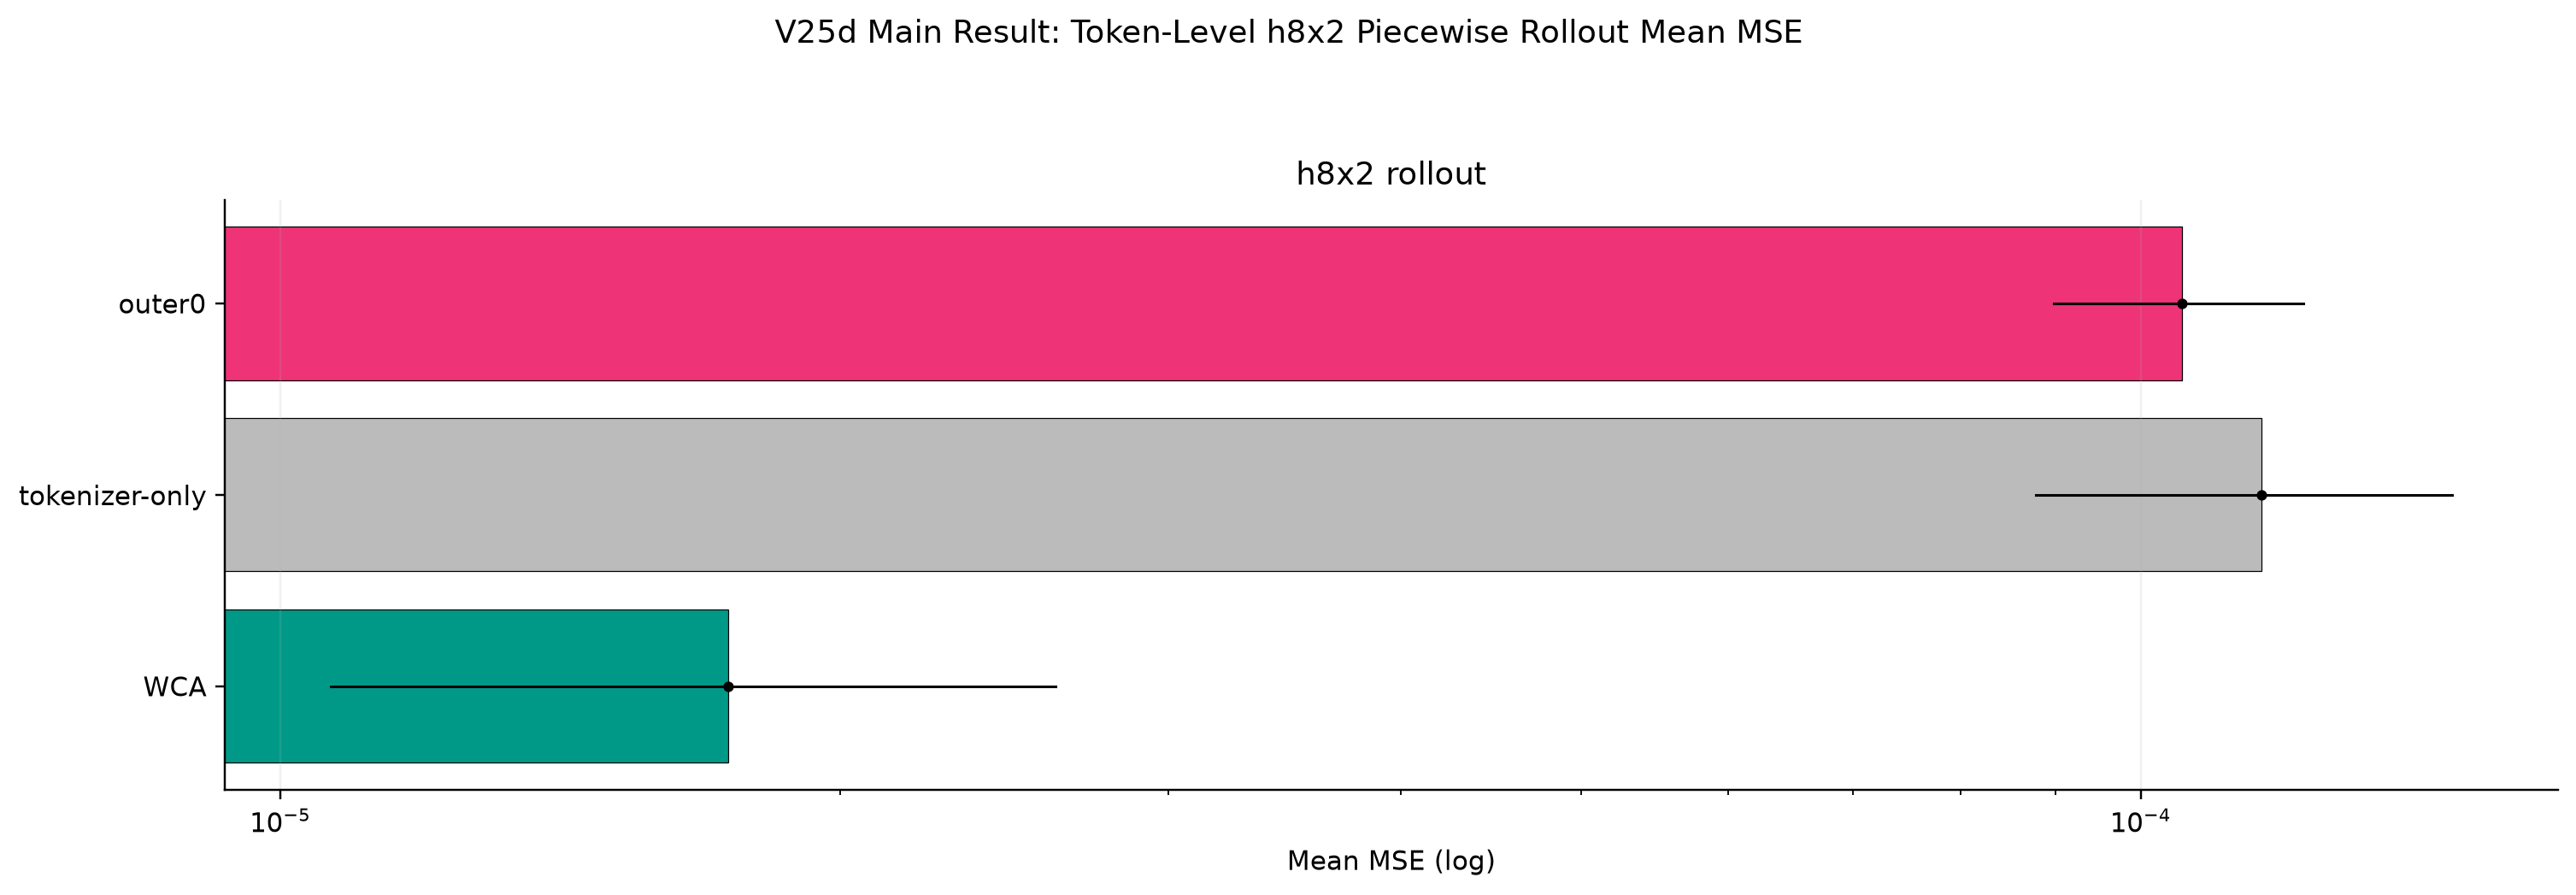
\includegraphics[width=0.86\linewidth]{v25d_rollout_mean_mse.png}
\caption{V25d h8x2 rollout mean MSE。主比较是 token-level WCA 与 same-family 控制组。}
\end{figure}

\begin{figure}[H]
\centering
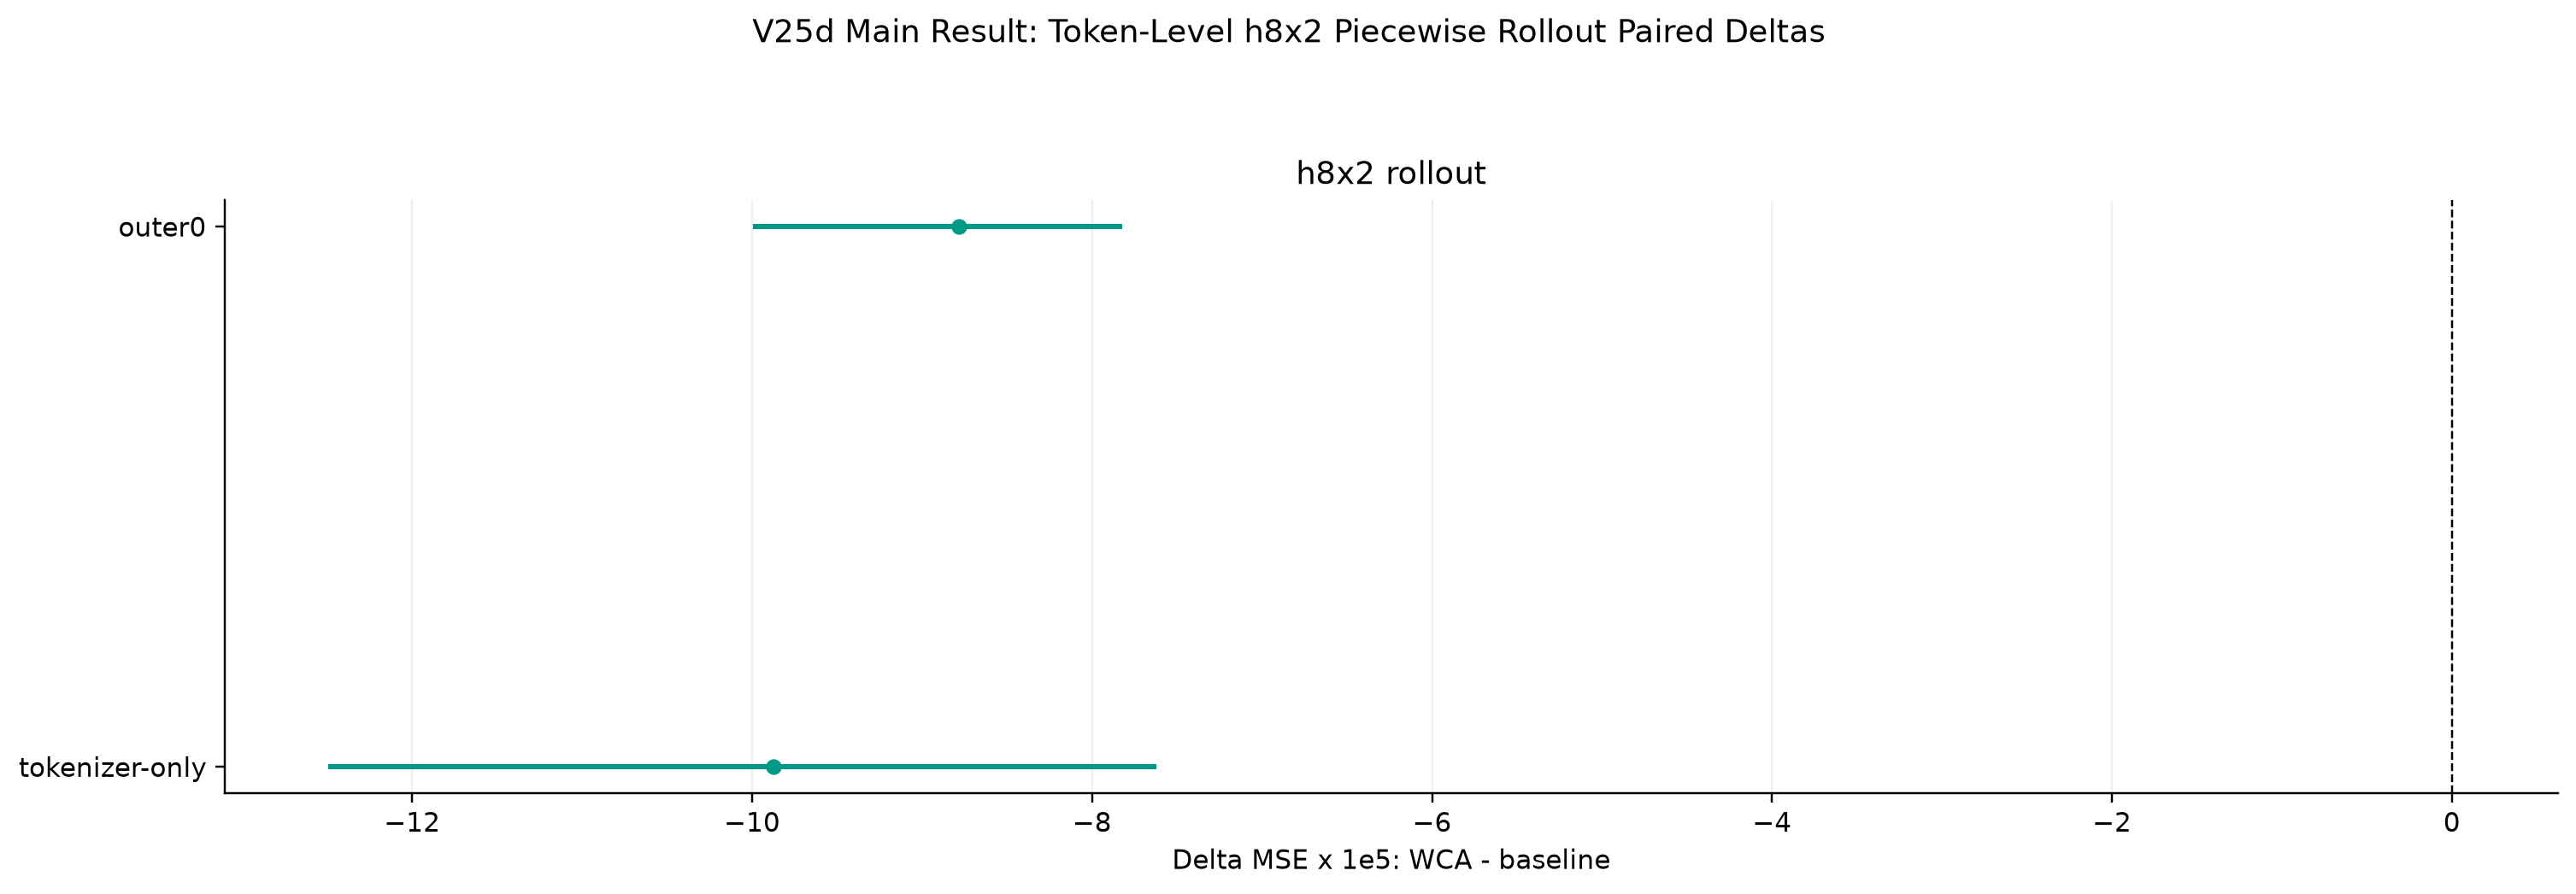
\includegraphics[width=0.86\linewidth]{v25d_rollout_paired_delta.png}
\caption{固定 starts 上的 paired rollout delta。该图支持 h8x2 token-level rollout 结论，但不能替代更多 seed 复验。}
\end{figure}

\section{定性图与 metric space 边界}

WCA token-level 输出通过 patch repetition 可视化，所以看起来更块状。这是表示边界，不是 metric 错误。raw/full-field FNO 或 U-Net 可以保留 patch 内细节，因此看起来更细腻。图像只能作为诊断，不能跨 metric space 直接证明谁更强。

\begin{figure}[H]
\centering
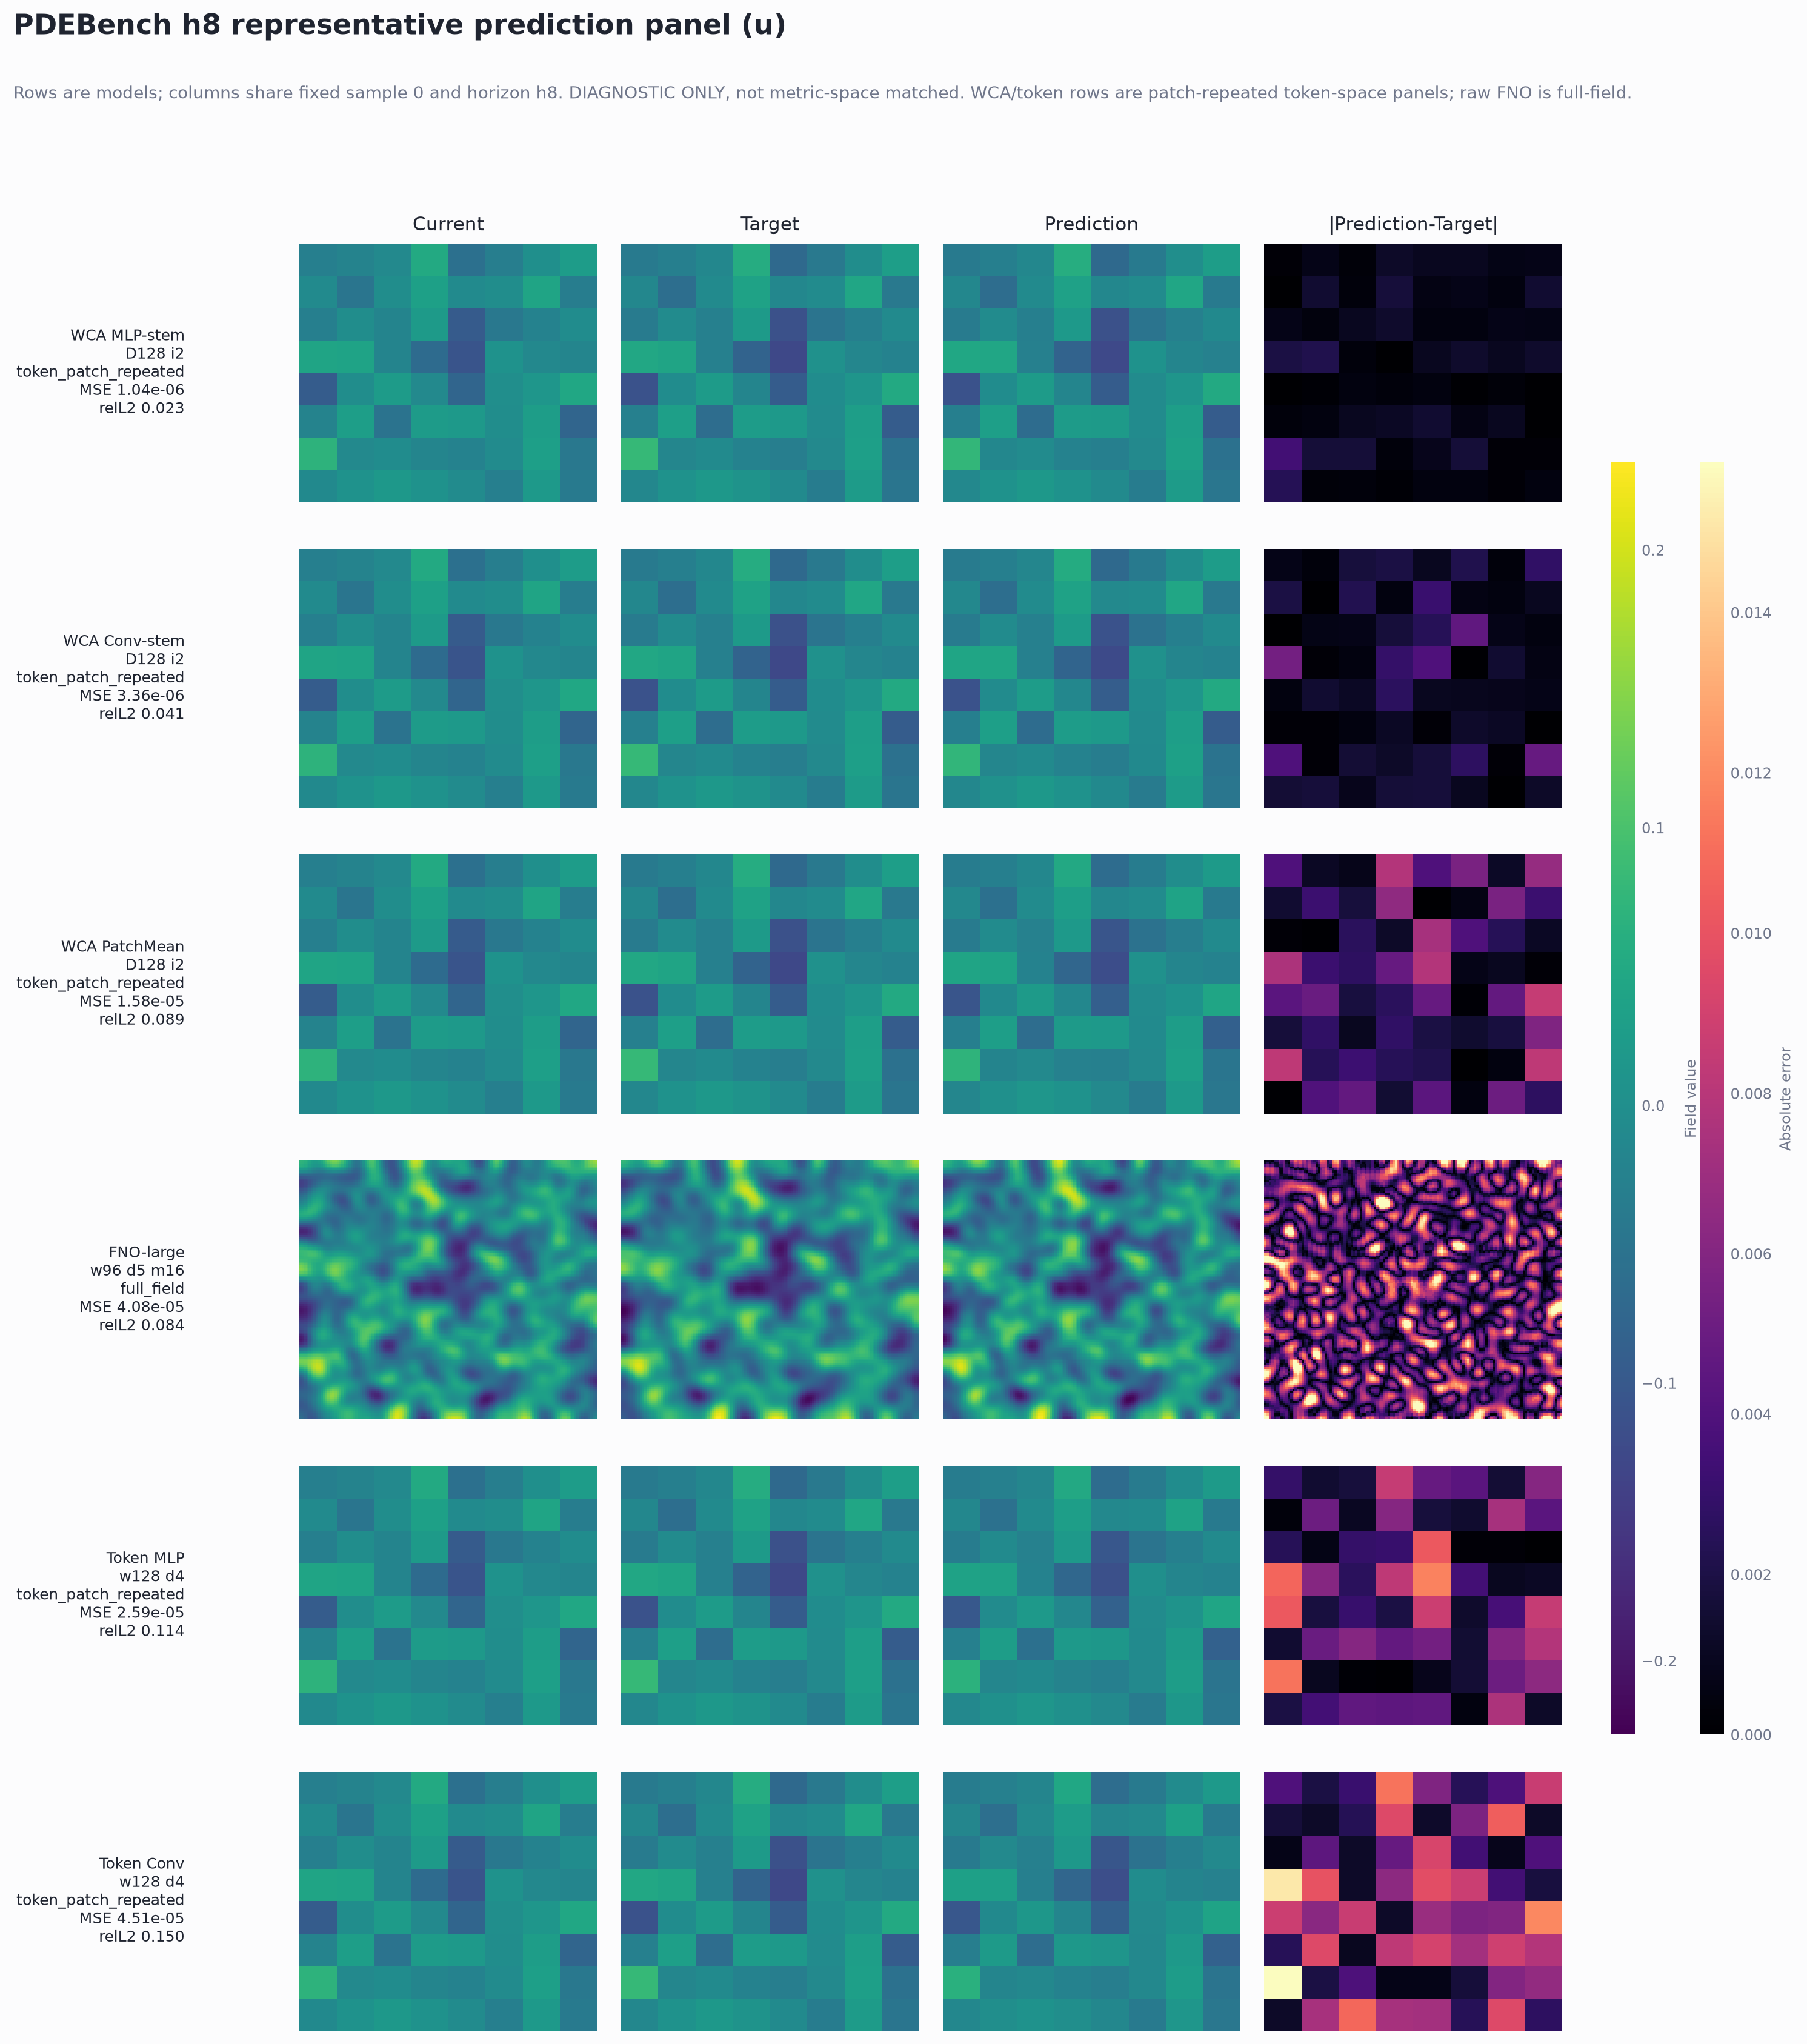
\includegraphics[width=0.95\linewidth]{pdebench_h8_u_model_composite.png}
\caption{PDEBench h8 channel $u$ 定性图。WCA/token 行是 patch-repeated token output。}
\end{figure}

\begin{figure}[H]
\centering
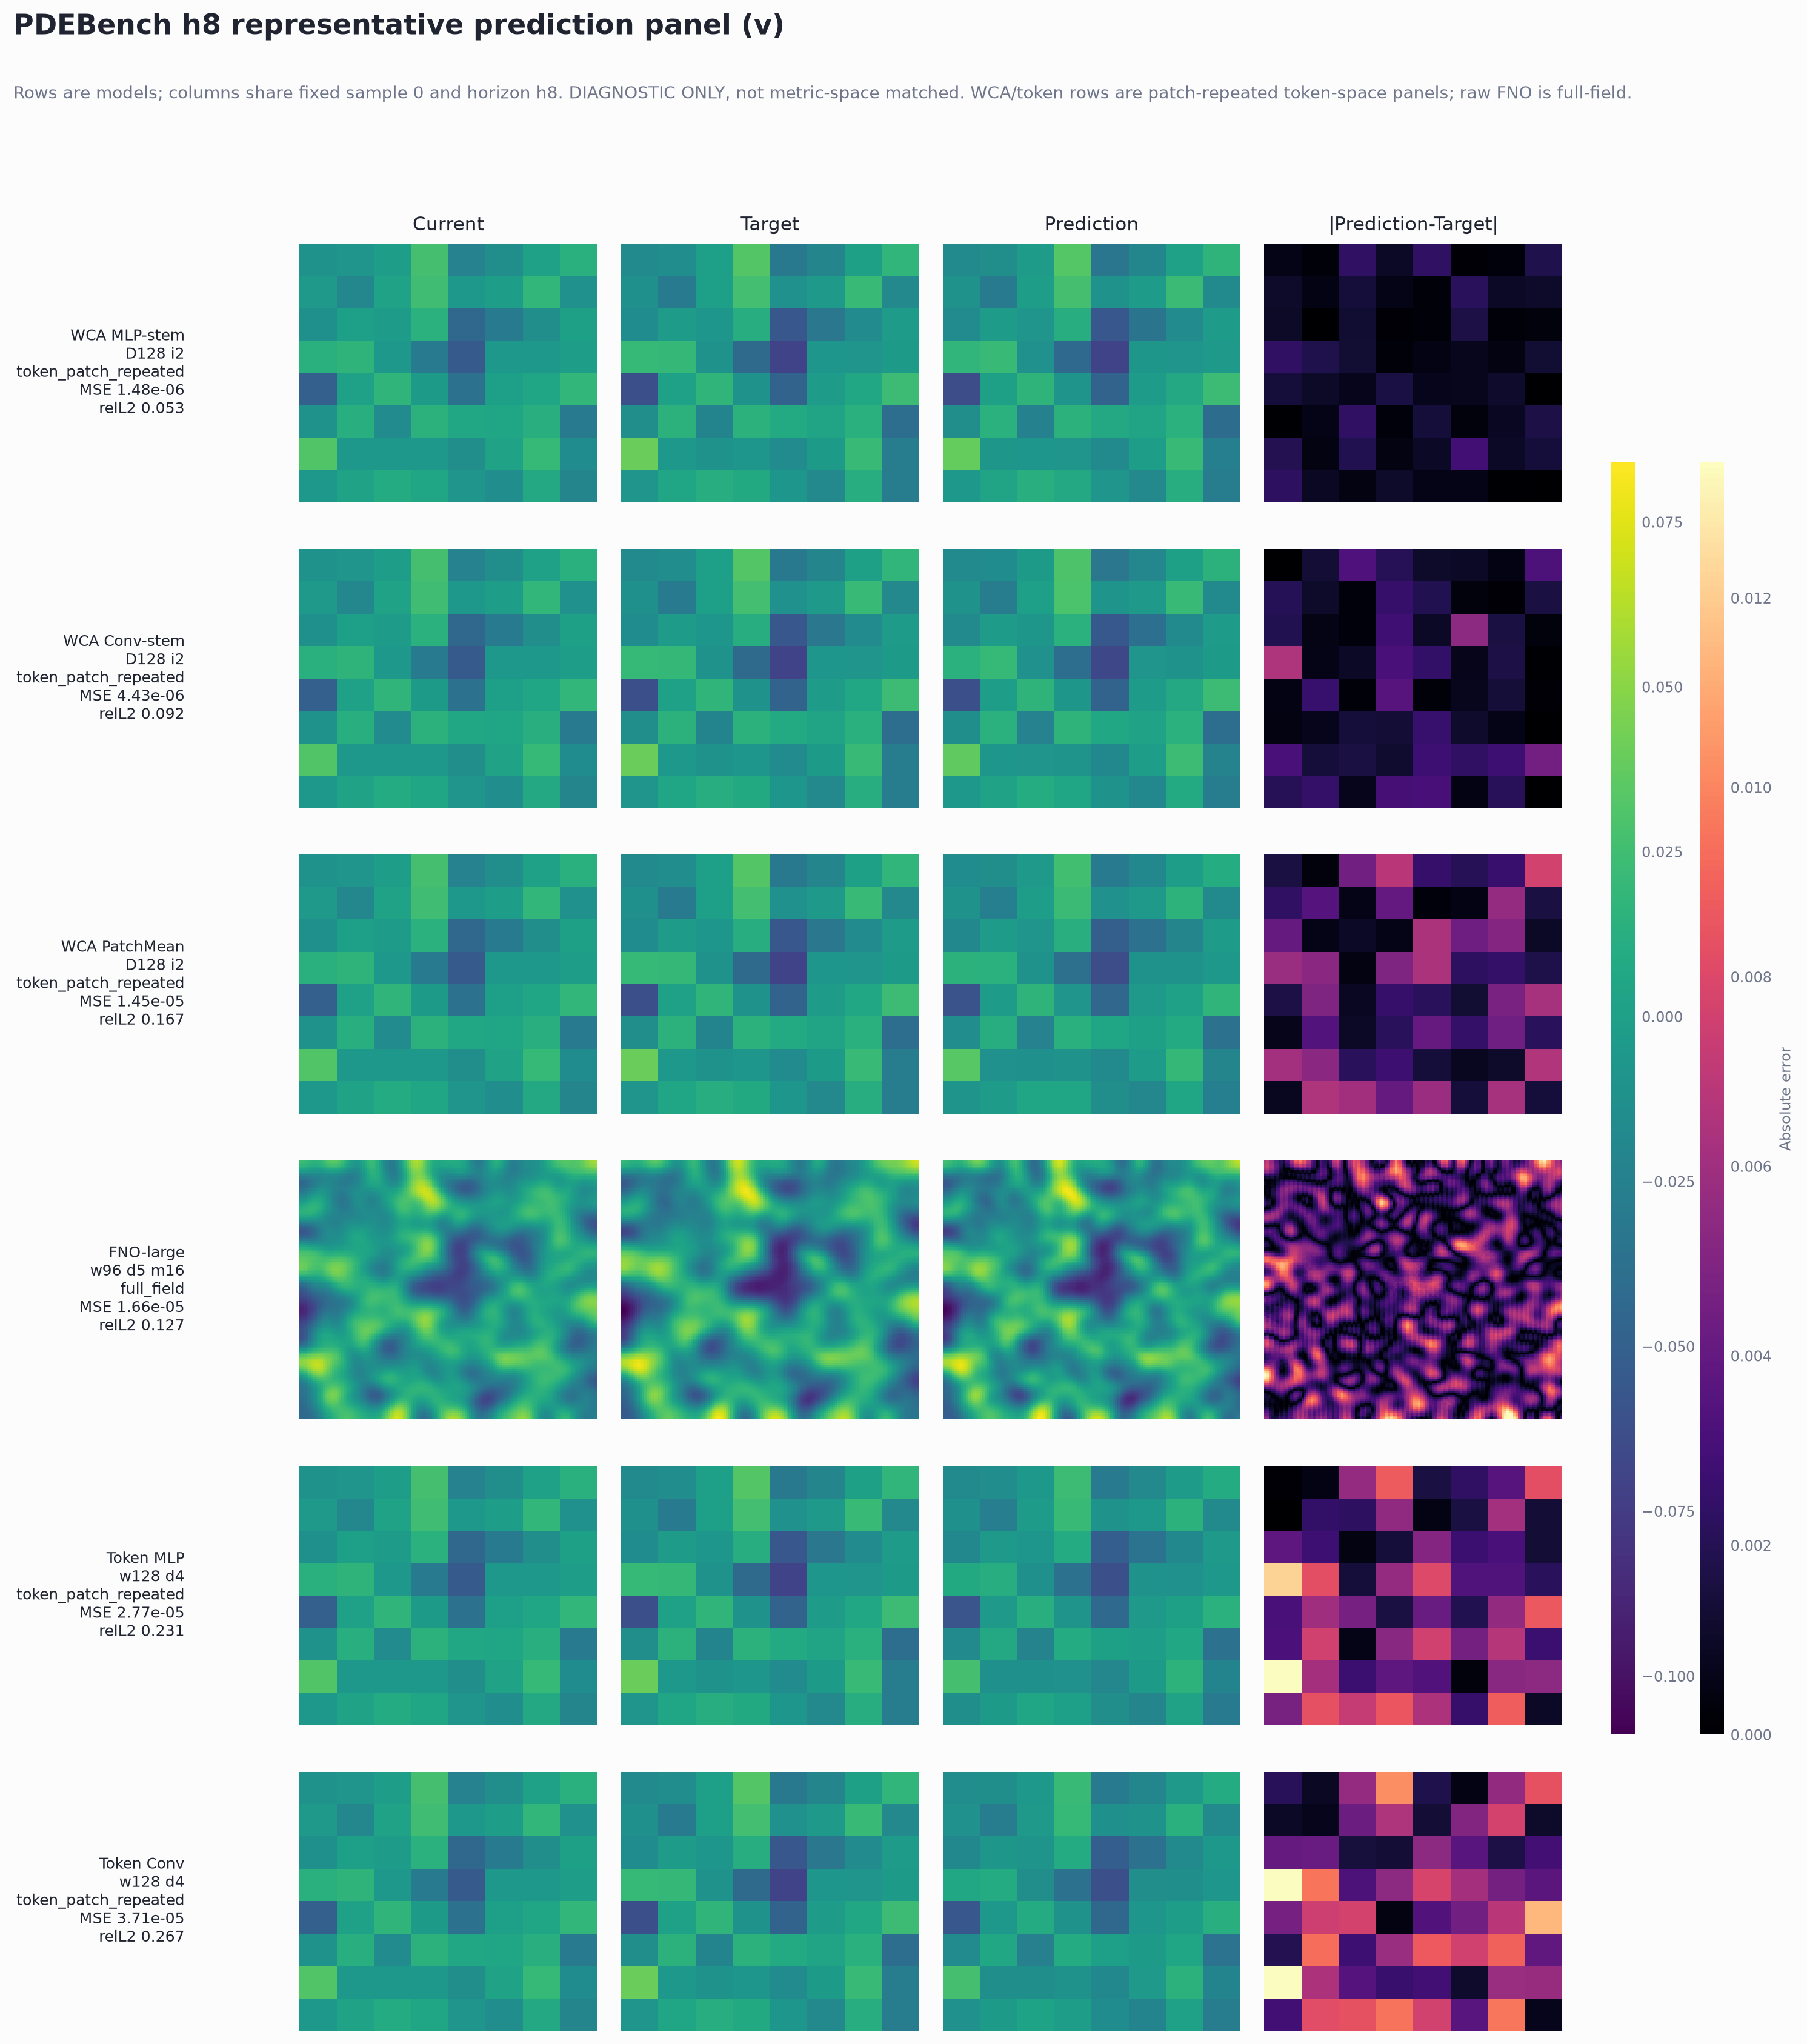
\includegraphics[width=0.95\linewidth]{pdebench_h8_v_model_composite.png}
\caption{PDEBench h8 channel $v$ 定性图。定量结论必须来自明确声明的 metric space。}
\end{figure}

\section{负结果与经验}

技术报告必须记录失败，因为失败定义下一步。

\subsection{Maze failure modes}

复杂 maze 暴露了 local minima、loop 和 shortcut learning。这说明 WCA 可以形成有用场，但导航任务仍需要 topology-aware loss 和 functional rollout metrics。

\subsection{PatchMean bottleneck}

PatchMean 简单可审计，但损失局部结构。它暴露了短期预测瓶颈，也推动了可学习接口分支。

\subsection{N=256 PatchMean boundary}

N=256 PatchMean WCA 弱于 matched token baselines。这不意味着 WCA 不能 scale，而是说明弱接口加 dense 实现会暴露容量和优化问题。下一步应使用 learnable interface 和 capacity-safe recursion ladder。

\subsection{Decoder 与 tokenizer confound}

可学习接口提升性能，也带来归因风险。大 decoder 可能变成独立模型。正确做法不是不用接口，而是加入 tokenizer-only、outer0、decoder-size 和 token-equivalent baseline。

\section{当前解释}

当前证据支持四点：

\begin{enumerate}[leftmargin=2em]
  \item WCA 是一个与 GNN、attention、direct neural operator 不同的清晰架构。
  \item PDEBench reaction-diffusion 中，递归深度对 h8 行为有帮助。
  \item 可学习接口显著释放 WCA 表现，source-audit 控制实验支持 WCA core 在若干 horizon 上的贡献。
  \item V25d h8x2 token-level rollout 是当前最干净的 formal 证据，说明 WCA core 可以支持迭代长程 token dynamics。
\end{enumerate}

这些证据还没有完成整个 world model 目标。native full-field decoding、更广 PDE family、更长 rollout、更强复验、高效 dense-equivalent kernel 和统一物理 latent 仍然是下一阶段工作。

\section{路线图}

\subsection{Native 与 learnable interface}

下一步需要更强 native field interface，既保留 patch 内信息，又不能让 decoder 偷偷承担全部预测。必须配套 interface ablation、decoder control 和 token-equivalent baseline。

\subsection{更多 PDE families}

Reaction-diffusion 只是一个物理族。下一阶段应加入 advection、Burgers、wave、diffusion variants 和 Navier-Stokes-like flows，只要它们有严格 split contract。

\subsection{更长 rollout}

h8x2 很有价值，但更强 world-state test 需要更长 rollout、spectrum/energy drift、native-resolution error 和稳定性诊断。

\subsection{高效 dense-equivalent 实现}

Full dense WCA 成本高。第一阶段系统目标不是改变数学，而是在保持 dense 语义的前提下提升显存和 GPU 吞吐。后续 sparse、hybrid、multiscale 都应作为显式变体并通过等价或 ablation gate。

\subsection{统一物理 latent}

长期方向是统一物理 latent。图像、触觉网格、仿真器状态、天气场、迷宫状态等都可以编码到共享 WCA state space。这不是当前结果，但它是 WCA 作为 state-space architecture 的自然延伸。

\section{复现与发布包}

公开发布包应包含：

\begin{itemize}[leftmargin=2em]
  \item 中英文技术报告；
  \item LaTeX 源文件和 PDF；
  \item 报告使用的图和表；
  \item 区分 formal、source-audit、secondary、diagnostic、future evidence 的 claim table；
  \item artifact manifest 和 hash；
  \item GitHub、Hugging Face、Zenodo 发布说明；
  \item 复现说明，包括 split、horizon、token、checkpoint contract。
\end{itemize}

\section{结论}

WCA 是一种面向世界状态建模的递归局部世界架构。它把全局状态展开成以中心节点索引的局部世界，在局部世界内部通过成对交互演化，再把演化中心重组成下一步全局状态。这个结构使 WCA 区别于普通 MLP、GNN message passing、Transformer attention 和 direct neural operator。

目前实验说明 WCA 值得继续深入研究。Maze 实验展示了 world-field 形成能力并暴露拓扑失败；WeatherBench-style 实验证明其能处理真实多变量场；PDEBench reaction-diffusion 给出了最强当前证据：递归深度有用，可学习接口释放更强动力学，h8x2 token-level rollout 支持 WCA core 相比 interface-only 和 no-recursion 控制组的贡献。

因此，WCA 应被发展为一种候选世界状态建模基底。下一步应围绕更严格归因、更强 native interface、更广物理 bench、更长 rollout 和高效 dense-equivalent 实现继续推进。

\end{document}
